\chapter{Choix d'un Modèle}\label{Ch-Model}
\begin{abstract}
L'intégralité de la méthode des éléments finis a été présentée au chapitre
précédent.

Avant de présenter plus en détail la formulation d'éléments finis,
nous tenions à ajouter un court chapitre comme mise en garde en
modélisation.
Comme ce document étant essentiellement destiné à un public d'ingénieurs mécaniciens,
nous allons illustrer notre propos en mécanique.
\end{abstract}

%Ce document étant essentiellement destiné à un public d'ingénieurs mécaniciens,
%nous allons illustrer notre propos en mécanique.




\medskip
\begin{histoire}%
La mécanique est sans doute aussi vieille que l'homme.
Aussi bien pour des aspects pratiques (faire des outils pour chasser...),
que pour des aspects plus philosophiques et spirituels visant notamment à 
expliquer les mouvements des astres... 

\sbox{\MaBoiteAvecPhotos}{\setlength{\tabcolsep}{0pt}\scriptsize%
\begin{tabular}{ccc}%
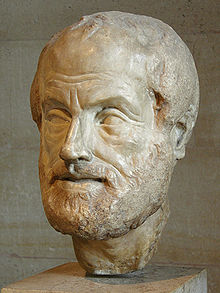
\includegraphics[height=\the\HauteurDesPhotos]{Aristote}&
\includegraphics[height=\the\HauteurDesPhotos]{Archimede2}&
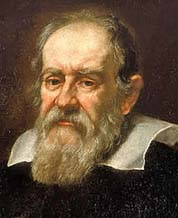
\includegraphics[height=\the\HauteurDesPhotos]{Galilee}\\
Aristote&Archimède&Galilée%
\end{tabular}}
\medskip
\ImageADroite{%
Archimède,\index[aut]{Archimède de Syracuse, -287-- -212, Grec} 
outre ces travaux en mathématiques, pourrait sans conteste être
considéré comme le saint patron de la mécanique. Il est tout au moins indubitablement
le père de la mécanique statique.\\
\indent
Il s'intéressa aussi bien aux aspects <<~théoriques~>> portant sur le principe 
du levier et la recherche de centre de gravité dans \emph{De l'équilibre des figures 
planes}, sur le principe d'Archimède sur les corps plongés dans un liquide 
dans \emph{Des corps flottants}; qu'aux aspects pratiques au travers de 
nombreuses inventions: machines de traction (où il démontre qu'à l'aide de poulies, 
de palans et de leviers, l'homme peut soulever bien plus que son poids), machines de guerre 
(principe de la meurtrière, catapultes, bras mécaniques utilisés dans le combat naval), 
l'odomètre (appareil à mesurer les distances), la vis sans fin et la vis d'Archimède,
le principe de la roue dentée...
}

Le siège de Syracuse, les miroirs d'Archmède et sa mort ne font qu'ajouter
à sa légende.


\medskip
Bien qu'Aristote\index[aut]{Aristote (dit le Stagirite), -384-- -322, Grec} 
posa le premier (avant Archimède)\index[aut]{Archimède de Syracuse, -287-- -212, Grec} 
les bases d'une véritable théorie mécanique (alors encore très imparfaite), les fondements 
de la mécanique, en tant que science et au sens moderne du terme, sont posés par Galilée\index[aut]{Galilée (Galileo Galilei), 1564-1642, Italien} 
en 1632 dans \emph{les Dialogues} et en 1638 dans \emph{les Discours}. 

La mécanique n'est alors pas dissociée des arts mécaniques, i.e. des techniques de 
construction des machines. 
La distinction entre la mécanique en tant science et la mécanique en tant que technique
ne se fera qu'au XIXe siècle.

\sbox{\MaBoiteAvecPhotos}{\setlength{\tabcolsep}{0pt}\scriptsize%
\begin{tabular}{c}%
\includegraphics[height=\the\HauteurDesPhotos]{Newton2}\\%
Newton%
\end{tabular}}
\medskip
\ImageADroite{%
En 1677, Newton\index[aut]{Newton (Isaac, Sir -), 1643-1727, Anglais} 
reprend ses travaux sur la mécanique, i.e. sur la gravitation et ses effets 
sur les orbites des planètes.
En novembre 1684, il fit parvenir à Halley\index[aut]{Halley (Edmond), 1656-1742, Anglais} 
un petit traité de neuf pages avec le titre: 
\emph{De motu corporum in gyrum} (Mouvement des corps en rotation), montrant la loi 
en carré inverse, la force centripète, ainsi que les prémices des lois du mouvement.\\
\indent
Son ouvrage \emph{Philosophi\ae Naturalis Principia Mathematica}
(aujourd'hui connu sous le nom de \emph{Principia} ou \emph{Principia Mathematica}),
écrit en 1686 et publié le 5 juillet 1687, 
est considéré comme une œuvre majeure dans l'histoire de la science. 
Il y décrit la gravitation universelle, formule les trois lois du mouvement et jette les bases 
de la mécanique classique ou mécanique newtonnienne. 
Ces trois lois universelles du mouvement resteront inchangées, sans aucune amélioration, 
durant plus de deux siècles, jusqu'à l'arrivée des mécaniques relativiste et quantique.
}

\medskip
Rappelons que ces trois lois sont: 1) le principe d'inertie; 2) le principe fondamental
de la dynamique; et 3) le principe des actions réciproques.

\medskip
La mécanique classique sera ensuite complétée et mathématisée pour devenir la
mécanique analytique.
Cette dernière, initiée dès le XVIIIe siècle, regroupe, en plus de la mécanique 
newtonienne,\index[aut]{Neumann (Carl Gottfried), 1832-1925, Allemand} les mécaniques 
de Hamilton\index[aut]{Hamilton (William Rowan, Sir -), 1805-1865, Irlandais} 
et de Lagrange.\index[aut]{Lagrange (Joseph Louis, comte de -), 1736-1813, Italien}
Toutes ces mécaniques ont en commun l'application initiale d'un principe variationnel, 
et avec lui l'utilisation du calcul variationnel... ce qui fait le lien avec le présent document.
\end{histoire}
\colorblack








\medskip
\section{La mécanique, un problème à plusieurs champs}\label{Sec-champs}

Dans ce paragraphe, nous reprenons les formulation présentées au paragraphe \ref{Sec-form},
mais en essayant de les éclairer par un discours plus pragmatique. C'est pourquoi nous
changerons quelque peu les notations, afin de retomber sur des choses peut-être plus familières
pour des ingénieurs mécaniciens.

\medskip
Bien qu'étant un sujet ancien, la mécanique n'en est pas pour autant un problème simple.

En mécanique, les champs inconnus sont les déplacements, déformations 
et contraintes (et d'autres si besoin, comme la température...). 
De plus, on dispose de relations entre ces champs.

\medskip
Il est possible de n'exprimer le problème qu'à l'aide des seuls déplacements.
Les déformations sont alors calculées à partir des déplacements (par combinaison
linéaire des dérivées, obtenues de manière approchée), puis les contraintes
sont obtenues à partir des déformations par la loi de comportement (linéaire ou non,
isotrope ou non...).

\medskip
Il est également tout à fait possible d'exprimer le problème en 
utilisant les déplacements et les contraintes comme inconnues. 
Cela permet de prendre en compte certaines continuités des contraintes en certains lieux 
(interface entre deux matériaux par exemple, voir paragraphe \ref{Sec-interf} pour une synthèse) 
de la structure, et d'imposer les CL de nullité des contraintes aux lieux le nécessitant (par exemple bord libre).

Par contre, le champ de contraintes peut également être <<~trop~>> continu
en certains endroits selon le type de problème. Cette continuité étant
liée à la constitution de l'élément fini choisi, on peut ne pas disposer
d'éléments capables de modéliser correctement ce phénomène...

\medskip
Notons qu'il serait tout aussi possible d'utiliser une formulation ayant les trois champs 
comme inconnues...

\textcolorred{Enfin bref, tout est possible, mais il faut veiller à ce que la modélisation de chaque
champ soit cohérente avec le phénomène physique à modéliser.}

\textcolorgreen{En d'autres termes, on ne choisit pas un élément au hasard, juste parce qu'il a le 
bon nombre d'inconnues, il est évidemment nécessaire de se demander comment 
ces inconnues sont interpolées, ce que cela implique sur la régularité des solutions 
et donc si cela est compatible avec le phénomène physique que l'on souhaite simuler.}

\medskip
Un autre exemple typique est le cas des éléments <<~déplacement-pression~>>
utilisés par exemple pour la modélisation des solides incompressibles (nous avons
évoqué le problème précédemment).



\bigskip
\textcolorred{Ce document s'adressant à des personnes connaissant déjà la MEF, nous allons
présenter très brièvement, sous forme d'a parte, la discrétisation multi-champs, de 
manière un peu découplée du reste du document, juste pour fixer les idées.}

\medskip
Si l'on note $u$ le champ de déplacements, il peut être approximé à partir
des déplacements nodaux (sous forme de vecteur) $\VV{q}$ par l'intermédiaire
de fonctions de formes rangées dans la matrice $\MM{N_u}$.

Compte tenu des notations utilisé{}es, les interpolations des diffé{}rents
champs se font, sur chaque é{}lé{}ment, de la maniè{}re suivante:
\begin{equation}
   u=\MM{N_u}\VV{q}
\end{equation}

De la même manière, si les dé{}formations $\varepsilon$ sont choisies comme champ inconnu,
elles seront approximées à partir des déformations nodales (sous forme de vecteur avec
la convention de l'ingénieur) $\VV{\gamma}$ par l'intermédiaire de fonctions de formes rangées 
dans la matrice $\MM{N_\varepsilon}$.
\begin{equation}
   \varepsilon = \MM{N_\varepsilon}\VV{\gamma}
\end{equation}

Cela vaut également pour les contraintes $\sigma$ qui, si elles sont choisies comme champ
inconnu, seront approximées à partir des contraintes nodales (sous forme de vecteur avec
la convention de l'ingénieur) $\VV{\tau}$ par l'intermédiaire de fonctions de formes rangées 
dans la matrice $\MM{N_\sigma}$.
\begin{equation}
   \sigma = \MM{N_\sigma}\VV{\tau}
\end{equation}

Notons que dans la pratique, rien n'empêche de prendre les mê{}mes fonctions
de forme pour les diffé{}rents champs.

\medskip
De maniè{}re analogue, le vecteur $\VV{\lambda}$ de multiplicateurs
de Lagrange sera interpolé{} de la fa\c{c}on suivante:
\begin{equation}
   \VV{\lambda}=\MM{N_\lambda}\VV{L}
\end{equation}

\medskip
On aura donc:\index[aut]{Hooke (Robert), 1635-1703, Anglais}
\begin{equation}
   \begin{array}{rcll}
   \varepsilon &=& \MM{N_\varepsilon}\VV{\gamma}
                      &\text{approximation en dé{}formations}\\
                    &=& \MM{\cL}u
                      &\text{relation dé{}formations dé{}placements}\\
                    &=& \MM{\cL}\MM{N_u}\VV{q}
                      &\text{approximation en dé{}placements}\\
                    &=& \MM{S}\sigma
                      &\text{loi de Hooke inverse}\\
                    &=& \MM{S}\MM{N_\sigma}\VV{\tau}
                      &\text{approximation en contraintes}
   \end{array}
\end{equation}
et, de fa\c{c}on inverse:\index[aut]{Hooke (Robert), 1635-1703, Anglais}
\begin{equation}
   \begin{array}{rcll}
   \sigma &=& \MM{N_\sigma}\VV{\tau}
                      &\text{approximation en contraintes}\\
                    &=& \MM{H}\varepsilon
                      &\text{loi de Hooke gé{}né{}ralisé{}e}\\
                    &=& \MM{H}\MM{N_\varepsilon}\VV{\gamma}
                      &\text{approximation en dé{}formations}\\
                    &=& \MM{H}\MM{\cL}u
                      &\text{loi de Hooke en é{}lasticité{} liné{}aire}\\
                    &=& \MM{H}\MM{\cL}\MM{N_u}\VV{q}
                      &\text{approximation en dé{}placements}
   \end{array}
\end{equation}
avec, en petites déformations:
\begin{equation}
   \MM{\cL} = \MMM{
                 \begin{array}{cc}
                    \tfrac{\partial}{\partial x} & 0\\
                    0 & \tfrac{\partial}{\partial y}\\
                    \tfrac{\partial}{\partial y} &
                    \tfrac{\partial}{\partial x}
                 \end{array}
              }
   \text{ en 2D, et }
   \MM{\cL} = \MMM{
                 \begin{array}{ccc}
                    \tfrac{\partial}{\partial x} & 0 & 0\\
                    0 & \tfrac{\partial}{\partial y} & 0\\
                    0 & 0 & \tfrac{\partial}{\partial z}\\
                    0 & \tfrac{\partial}{\partial z} &
                    \tfrac{\partial}{\partial y}\\
                    \tfrac{\partial}{\partial z} & 0&
                    \tfrac{\partial}{\partial x} \\
                    \tfrac{\partial}{\partial y} &
                    \tfrac{\partial}{\partial x} &0\\
                 \end{array}
              }
   \text{ en 3D}
\end{equation}

\medskip
La mé{}thode des é{}lé{}ments finis \emph{classique}, ou \emph{en
dé{}placements}, n'utilise que le champ de dé{}placements comme
variable. Elle est basé{}e sur le \textcolorblue{principe du travail virtuel}:
\begin{equation}
   \label{Eq:deltaPiTV}
   \delta\Pi_{TV} = \dint_{\Omega} \delta\varepsilon(u)H\varepsilon(u)
           - \delta u\fbar \ \dd\Omega
           -\dint_{\ls} \delta u\Tbar \ \dd\Gamma
\end{equation}
avec $\fbar$ les forces imposées dans $\Omega$ et $\Tbar$ les forces imposées
sur $\ls$, où $\ls$ et $\lu$ forment une partition de
$\Gamma=\partial\Omega$.

\medskip
Ce principe est obtenu comme variation de la fonctionnelle de
l'\textcolorblue{é{}nergie potentielle totale} exprimé{}e en dé{}placements:
\begin{equation}
   \label{Eq:PiTV}
   \Pi_{TV} = \dint_{\Omega} \tfrac12 \LL{\varepsilon(u)}\MM{H}\VV{\varepsilon(u)}
           - \LL{q}\VV{\fbar} \ \dd\Omega
           -\dint_{\ls} \LL{q}\VV{\Tbar} \ \dd\Gamma
\end{equation}
où les conditions subsidiaires sur les dé{}placements sont prises en compte
directement par l'espace dans lequel les déplacements sont recherchés.

\medskip
La \textcolorblue{fonctionnelle d'Hellinger-Reissner}\index[aut]{Hellinger}
\index[aut]{Reissner (Max Erich, dit Eric), 1913-1996, Américain} est sans doute la plus
connue des fonctionnelles mixtes. Elle utilise les champs de
dé{}placements et de contraintes comme variables indé{}pendantes.
Son expression est la suivante, $\Ubar$ désignant les déplacement imposés:
\begin{equation}
   \label{Eq:PiHR}
   \Pi_{HR}= \dint_\Omega -\tfrac12\sigma S\sigma
         - \sigma_{ij,j}u+ \fbar u\ \dd\Omega
        -\dint_{\ls} \left(\Tbar-T\right)u\ \dd\Gamma
         -\dint_{\lu} \Ubar T\ \dd\Gamma
\end{equation}
bien que l'on puisse la trouver sous une autre forme, obtenue par
inté{}gration par parties de celle-ci. Elle n'a à{} satisfaire
à{} aucune condition subsidiaire.

La stationnarité{} de cette fonctionnelle conduit aux é{}quations
d'é{}quilibre, à{} la loi de comportement, et aux conditions aux limites
en forces et déplacements.

\medskip
Cette fonctionnelle conduit à{} un é{}lé{}ment ayant les champs de
dé{}placements et de contraintes comme inconnues nodales. Il s'en
suit que toutes les composantes de ces champs sont continues.
Elle conduit à{} la ré{}solution d'un systè{}me du type mixte (Brezzi):\index[aut]{Brezzi (Franco), 1945-, Italien}
\begin{equation}
   \label{Eq:SysMixte}
   \MMM{\begin{array}{cc}
      -\MM{A} & \MM{B}\\
      \MM{B}^\TR &\mO
   \end{array}}
   \VVV{\begin{array}{c} \VV{\tau}\\\VV{q}\end{array}} =
   \VVV{\begin{array}{c} \mO\\\VV{F}\end{array}}
\end{equation}
où{} la matrice de rigidité{} est symé{}trique et non dé{}finie-positive, et:
\begin{equation}
   \MM{A}=+\dint_\Omega \MMT{N_\sigma}\MM{S}\MM{N_\sigma}\ \dd\Omega
   \qquad
   \MM{B}=+\dint_\Omega \MMT{N_\sigma}\MM{\cL}\MM{N_u}\ \dd\Omega
   \qquad
   \VV{F}=+\dint_\Omega \MMT{N_u}\VV{\fbar}\ \dd\Omega
\end{equation}

\medskip
L'un des moyens pour obtenir une fonctionnelle hybride est
d'introduire une condition sur une partie du contour par
l'intermé{}diaire de multiplicateurs de Lagrange comme pré{}senté{}
un peu plus loin.\index[aut]{Lagrange (Joseph Louis, comte de -), 1736-1813, Italien}

\medskip
Tout comme la fonctionnelle d'Hellinger-Reissner est associé{}e à{}
la mé{}thode mixte, celle de \textcolorblue{Pian et Tong}\index[aut]{Pian (Theodore H.H.), 1919-2009, Américain}\index[aut]{Tong (Pin), ? , Chinois}
 est indissociable
de l'adjectif \textcolorblue{hybride}, mê{}me si, en toute rigueur, elle est
une méthode mixte (deux champs) hybride (différents domaines
d'interpolation):
\begin{equation}
   \label{Eq:PiPT}
   \Pi_{PT} = -\tfrac12\dint_\Omega \sigma S\sigma\ \dd\Omega
         +\dint_{\Gamma} T u\ \dd\Gamma\\
         -\dint_{\ls} \Tbar u\ \dd\Gamma
\end{equation}

\medskip
Sa variation est:
\begin{equation}
   \label{Eq:deltaPiPT}
   \delta\Pi_{PT} =
        -\dint_{\Omega} \sigma S\sigma\ \dd\Omega
        +\dint_{\Gamma} \delta Tu+\delta uT\ \dd\Gamma
        -\dint_{\ls} \delta u \Tbar\ \dd\ls
\end{equation}
\textcolorgreen{dont l'avantage principal est de ne pas comporter de dé{}rivé{}e.}

\medskip
Cette variation peut ê{}tre transformé{}e en:
\[
   \dint_\Omega \delta \sigma (\varepsilon- S\sigma) \ \dd\Omega
   +\dint_{\Gamma} \delta uT\ \dd\Gamma
   -\dint_{\ls} \delta u\Tbar\ \dd\Gamma
\]
%ou encore:
%\[
%   \dint_\Omega \delta \sigma (\varepsilon-[S]\sigma) \ \dd\Omega
%   +\dint_{\ls} \delta u(T-\Tbar)\ \dd\Gamma\\
%   +\dint_{\li} \delta u(T^1+T^2)\ \dd\Gamma
%\]
%où{} les champs seront diffé{}rencié{}s par leur indice supé{}rieur ~$^1$ et
%~$^2$ de chaque c\o{}té{} de l'interface $\li$.

\medskip
La stationnarité{} de cette fonctionnelle conduit à{} la loi de
comportement, et aux conditions aux limites en contraintes. 
Les conditions aux limites en dé{}placements seront imposées par l'espace
dans lequel on cherche $u$.

\medskip
Le systè{}me à{} ré{}soudre est de la forme mixte donné{} précédemment à la relation (\ref{Eq:SysMixte})
avec:
\begin{equation}
   \MM{A} = +\dint_{\Omega} \MMT{N_\sigma}\MM{S}\MM{N_\sigma}\ \dd\Omega
\qquad
   \MM{B} = +\dint_{\Gamma} \MMT{N_\sigma}\MMT{M}\MM{N_u}\ \dd\Gamma
\qquad
   \VV{F} = +\dint_{\ls} \MMT{N_u}\VV{\Tbar} \ \dd\Gamma
\end{equation}
$\MM{M}$ é{}tant la matrice des cosinus directeurs donné{}e
par les relations:
\begin{equation}
%   \label{Eq:MatriceCosinusii}
   \MM{M}=\MMM{\begin{array}{ccc}
                  n_1&  0&n_2\\
                    0&n_2&n_1
                \end{array}}
%\end{equation}
\text{ dans le plan, et }%\\[-1.5ex]
%\begin{equation}
%   \label{Eq:MatriceCosinusiii}
   \MM{M}=\MMM{\begin{array}{cccccc}
                  n_1&  0&  0&  0&n_3&n_2\\
                    0&n_2&  0&n_3&  0&n_1\\
                    0&  0&n_3&n_2&n_1&  0
                \end{array}}
\text{ dans l'espace.}
\end{equation}

\bigskip
Toutefois, le champ de contraintes n'é{}tant dé{}fini que dans $\Omega$,
il est possible d'effectuer une \textcolorblue{condensation statique} du
champ de contraintes, i.e. de transformer le systè{}me
(\ref{Eq:SysMixte}) en é{}crivant:
\begin{equation}
   \label{Eq:TauQ}
      \VV{\tau} = \MMI{A}\MM{B}\VV{q}
\end{equation}
et le champ de dé{}placements est solution d'un systè{}me de type
classique $\MM{K}\VV{q}=\VV{F}$, où{} la matrice de rigidité $\MM{K}$ est remplacé{}e
par la matrice de rigidité{} é{}quivalente suivante:
\begin{equation}
%   \label{Eq:Keq}
   \MM{K_{eq}} = \MMT{B}\MMI{A}\MM{B}
\end{equation}


\medskip
Sur le plan du dé{}roulement du calcul, on commence par résoudre une <<~ forme classique ~>>
mais en utilisant la matrice de rigidité{} é{}quivalente $\MM{K_{eq}}$, puis le
calcul des contraintes dans chaque é{}lé{}ment se fait par la relation (\ref{Eq:TauQ}).


\bigskip
Les multiplicateurs de Lagrange\index[aut]{Lagrange (Joseph Louis, comte de -), 1736-1813, Italien} 
peuvent ê{}tre utilisé{}s pour introduire
des conditions supplé{}mentaires directement à{} la fonctionnelle.
Ces conditions sont gé{}né{}ralement imposé{}es sur $\Gamma_X$, tout ou
partie de $\Gamma$, contour de $\Omega$.
Pour ce faire, il suffit d'ajouter à{} la fonctionnelle $\Pi$
du problè{}me le terme:
\begin{equation}
   \pm\dint_{\Gamma_X} \LL{\lambda}\VV{\text{condition}}
\end{equation}
où{} les $\lambda_i$ sont les multiplicateurs de Lagrange.\index[aut]{Lagrange (Joseph Louis, comte de -), 1736-1813, Italien}

\medskip
Les multiplicateurs de Lagrange\index[aut]{Lagrange (Joseph Louis, comte de -), 1736-1813, Italien} 
sont gé{}né{}ralement utilisé{}s pour:
\begin{itemize}
   \item introduire des variables physiques additionnelles comme
         inconnues;
   \item obtenir des conditions de dé{}rivabilité{} ou des conditions aux
         limites moins sé{}vè{}res sur les inconnues.
\end{itemize}

\medskip
Notons qu'un autre de leurs avantages est de permettre l'utilisation d'une formulation diffé{}rente 
dans chaque é{}lé{}ment, en assurant les continuité{}s né{}cessaires aux interfaces (voir synthèse 
de ce problème d'interface au paragraphe \ref{Sec-interf}).
Bien sûr, apparaissant comme inconnues, ils viennent grossir la taille du systè{}me à
résoudre.










\medskip
\section{Plusieurs modélisations d'un même problème}\label{Sec-PlusModel}

La qualité de l'approximation des différents champs est non seulement liée
au nombre de champs inconnus choisis, mais également au choix de l'élément.
Ce dernier peut traduire une <<~simplification~>> du problème physique: 
il s'agit du problème du choix du type de modélisation, en 1, 2 ou 3D.

\textcolorred{Selon le type d'information recherché, un modélisation
<<~plus simple~>> qu'une autre peut fournir les résultats escomptés}.

\medskip
Dans ce paragraphe, nous nous proposons d'étudier un exemple où
\textcolorred{seul le champ de déplacement apparaît comme inconnue nodale}.
Toutefois, si ce n'est plus le nombre de champ qui peut modifier la formulation,
nous allons voir que la mécanique offre moult théories qui toutes ont leurs
avantages et inconvénients, mais qui surtout \textcolorred{ne sont pas toutes équivalentes.}

\bigskip
\begin{histoire}%
La paternité de la théorie des poutres est attribuée à Galilée,\index[aut]{Galilée (Galileo Galilei), 1564-1642, Italien} 
mais des études récentes indiquent que Léonard de Vinci\index[aut]{Vinci (Léonard, de-), 1452-1519, Italien} l'aurait précédé. 
De Vinci\index[aut]{Vinci (Léonard, de-), 1452-1519, Italien} avait supposé que la déformation 
variait de manière linéaire en s'éloignant de la surface neutre, le coefficient de proportionnalité 
étant la courbure, mais il ne put finaliser ses calculs car il n'avait pas imaginé la loi de Hooke\footnotemark.
De son côté, Galilée\index[aut]{Galilée (Galileo Galilei), 1564-1642, Italien} était parti sur 
une hypothèse incorrecte (il supposait que la contrainte était répartie uniformément en flexion), 
et c'est Antoine Parent\index[aut]{Parent (Antoine), 1660-1726, Français} qui obtint la distribution 
correcte.

\sbox{\MaBoiteAvecPhotos}{\setlength{\tabcolsep}{0pt}\scriptsize%
\begin{tabular}{cccc}
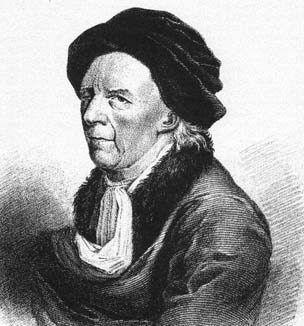
\includegraphics[height=\the\HauteurDesPhotos]{Euler5}&
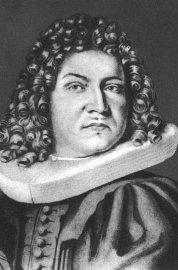
\includegraphics[height=\the\HauteurDesPhotos]{Bernoulli-Jacques}&
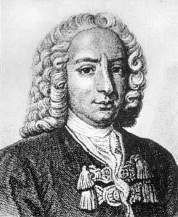
\includegraphics[height=\the\HauteurDesPhotos]{Bernoulli-Daniel}&
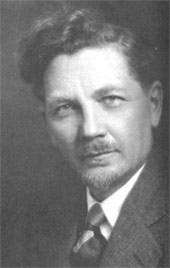
\includegraphics[height=\the\HauteurDesPhotos]{Timoshenko}\\
Euler&J. Bernoulli&D. Bernoulli&Timoshenko%
\end{tabular}}
\medskip
\ImageADroite{%
Ce sont Leonhard Euler\index[aut]{Euler (Leonhard Paul), 1707-1783, Suisse} et 
Jacques Bernoulli\index[aut]{Bernoulli (Jacques), 1654-1705, Suisse} qui émirent 
la première théorie utile vers 1750, tandis que Daniel Bernoulli,\index[aut]{Bernoulli (Daniel), 1700-1782, Suisse} 
le neveu du précédent (et le fils de Jean Bernoulli\index[aut]{Bernoulli (Jean), 1667-1748, Suisse}), 
écrivit l'équation différentielle pour l'analyse vibratoire. 
À cette époque, le génie mécanique n'était pas considéré comme une science, 
et l'on ne considérait pas que les travaux d'une académie des mathématiques puissent 
avoir des applications pratiques... On continua donc à bâtir les ponts et les bâtiments de 
manière empirique. 
Ce n'est qu'au XIXe siècle, avec la Tour Eiffel\index[aut]{Eiffel (Gustave), 1832-1923, Français} 
et les grandes roues, que l'on démontra la validité de la théorie à grande échelle.
}

\medskip
La théorie des poutres est une simplification unidimensionnelle. 
On distingue:
\begin{itemize}
   \item la théorie d'Euler-Bernoulli, qui néglige l'influence du cisaillement;
   \item la théorie de Timoshenko\index[aut]{Timoshenko (Stephen), 1878-1972, Russe} qui prend en compte l'effet du cisaillement.
\end{itemize}


\sbox{\MaBoiteAvecPhotos}{\setlength{\tabcolsep}{0pt}\scriptsize%
\begin{tabular}{cccc}
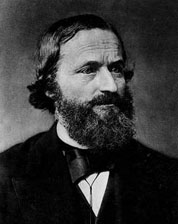
\includegraphics[height=\the\HauteurDesPhotos]{Kirchhoff}&
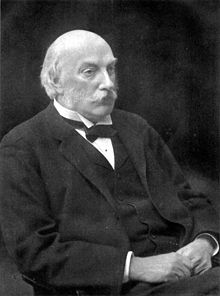
\includegraphics[height=\the\HauteurDesPhotos]{Rayleigh}&
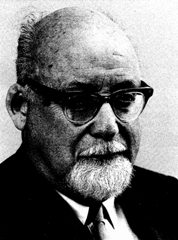
\includegraphics[height=\the\HauteurDesPhotos]{Reissner}&
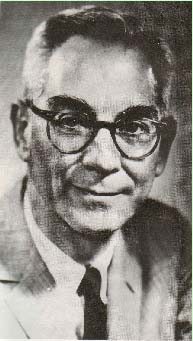
\includegraphics[height=\the\HauteurDesPhotos]{Mindlin}\\
Kirchhoff&Rayleigh&Reissner&Mindlin%
\end{tabular}}
\bigskip
\ImageAGauche{%
En 1888, Love\index[aut]{Love (Augustus Edward Hough), 1863-1940, Anglais} utilise 
les hypothèses de Gustav Kirchhoff,\index[aut]{Kirchhoff (Gustav Robert), 1824-1887, Allemand} 
elles-mêmes inspirées des hypothèses d'Euler-Bernoulli\index[aut]{Euler (Leonhard Paul), 1707-1783, Suisse}\index[aut]{Bernoulli (Jacques), 1654-1705, Suisse} pour les poutres, pour fonder une théorie des plaques minces.\\
La théorie des plaques épaisses a été consolidée par Mindlin\index[aut]{Mindlin (Raymond David), 1906-1987, Américain} 
à partir des travaux de Rayleigh (1877),\index[aut]{Rayleigh (John William Strutt, troisième baron -), 1842-1919, Anglais}
Timoshenko (1921),\index[aut]{Timoshenko (Stephen), 1878-1972, Russe} 
Reissner (1945)\index[aut]{Reissner (Max Erich, dit Eric), 1913-1996, Américain} 
et Uflyand (1948).\index[aut]{Uflyand (Yakov Solomonovic), ,Russe}
}

\medskip
La théorie des plaques minces, ou théorie de Love-Kirchhoff, suppose que:\index[aut]{Love (Augustus Edward Hough), 1863-1940, Anglais}\index[aut]{Kirchhoff (Gustav Robert), 1824-1887, Allemand}
\begin{itemize}
   \item le plan moyen (équivalent de la courbe moyenne des poutres) est initialement plan ;
   \item le feuillet moyen (équivalent de la fibre neutre des poutres) ne subit pas de déformation 
	dans son plan; on ne considère que le déplacement transversal $w$ des points du feuillet moyen ;
   \item modèle de Kirchhoff:\index[aut]{Kirchhoff (Gustav Robert), 1824-1887, Allemand} 
	les sections normales au feuillet moyen restent normales lors de la 
	déformation ; en conséquence, on peut négliger le cisaillement ;
   \item l'épaisseur est faible; en conséquence, les contraintes dans le sens de l'épaisseur sont 
	supposées nulles ;
   \item on reste en petites déformations.
\end{itemize}
Notons que cette théorie permet de déterminer la propagation des ondes dans les plaques, 
ainsi que l'étude des ondes stationnaires et des modes vibratoires. 

\medskip
Dans la théorie des plaques épaisses, ou théorie de Reissner\index[aut]{Reissner (Max Erich, dit Eric), 1913-1996, Américain} 
et Mindlin,\index[aut]{Mindlin (Raymond David), 1906-1987, Américain} la fibre normale reste 
toujours rectiligne, mais n'est plus nécessairement perpendiculaire au plan moyen.
On ne peut donc plus négliger le cisaillement.
%\footnote{%
%\begin{tabular}{ccccc}
%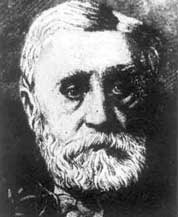
\includegraphics[height=32mm]{Saint-Venant}\\
%Claude Barré de Saint-Venant\\
%1797-1886\\
%\end{tabular}
%}
\footnotetext{%\colormagenta
Robert Hooke, qui désirait obtenir une théorie des ressorts en soumettant ces derniers à des forces 
croissantes successives, énonça en 1978, à partir d'expériences datant de 1675, 
la loi  de comportement suivante:
\og ut tensio sic vis \fg{}
ce qui signifie \og telle extension, telle force\fg{}, ou bien en termes modernes \og l'allongement est 
proportionnel à la force\fg{}.\colorblack}\index[aut]{Hooke (Robert), 1635-1703, Anglais}
\end{histoire}

\colorblack
\bigskip
La figure \ref{Pout1} propose trois modélisations d'un même problème.
Il s'agit d'une poutre encastrée \ a une extrémité et soumise \ a une force
décentrée \ a l'autre.
Vaut-il mieux modéliser l'intégralité du volume de la poutre, la traiter comme
une plaque, ou peut-on se contenter d'un modèle de poutre?
\begin{figure}[ht]
\begin{center}
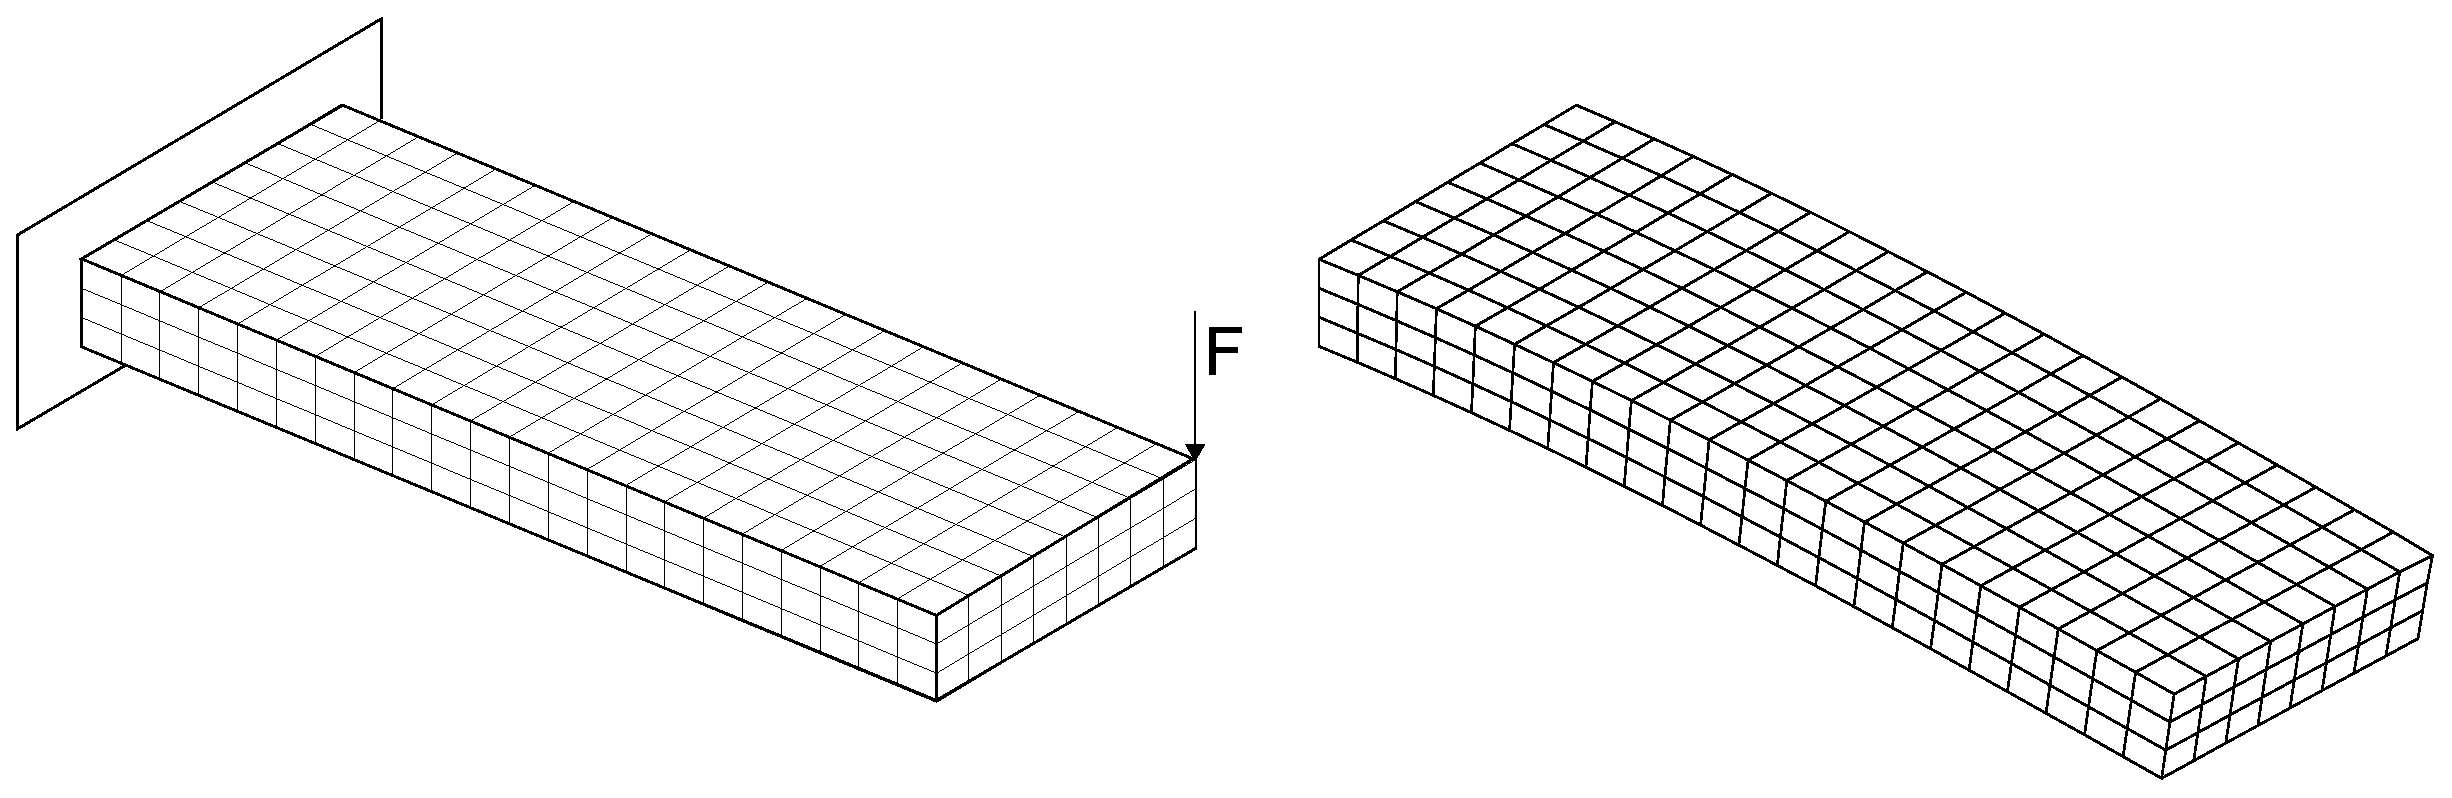
\includegraphics[height=14mm]{Pout1-3D.eps} \hfill
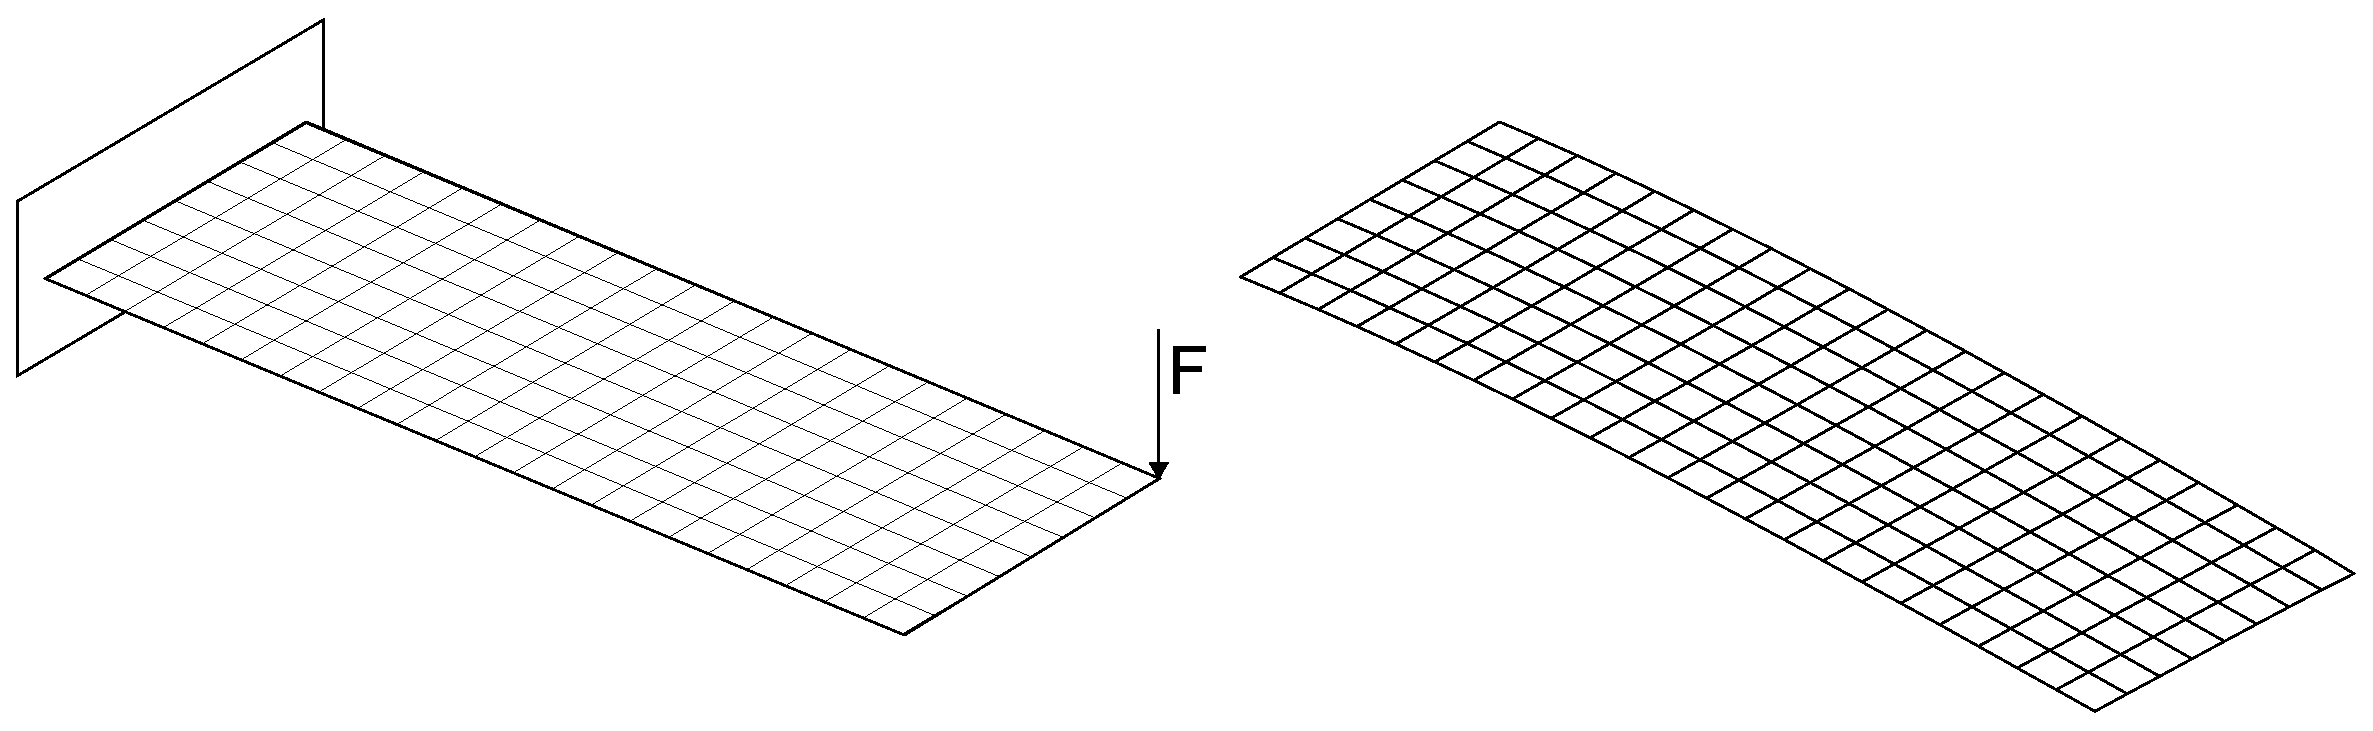
\includegraphics[height=14mm]{Pout1-2D.eps} \hfill
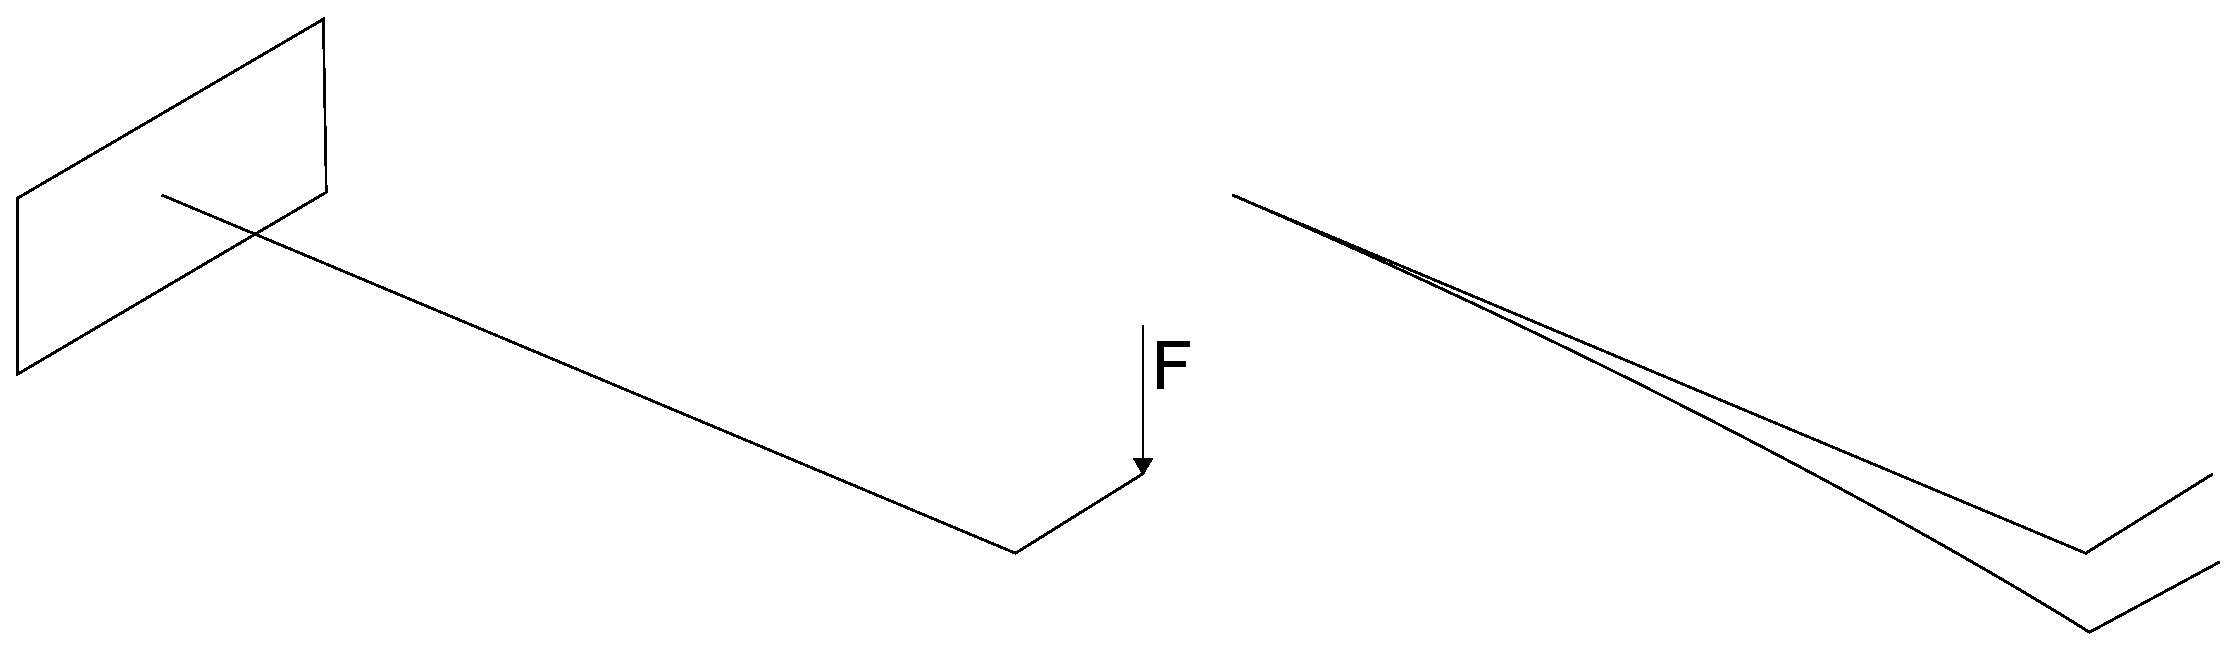
\includegraphics[height=14mm]{Pout1-1D.eps}
\end{center}
\caption{\label{Pout1} Trois modélisations d'un même problème.}
\end{figure}

\medskip
L'étude de la contrainte axiale $\sigma_{xx}$ est donnée à la figure \ref{Pout1-sigxx}.
\begin{figure}[ht]
\begin{center}
\includegraphics[height=45mm]{pout1-sigxx.eps}\\[-3mm]
\end{center}
\caption{\label{Pout1-sigxx} Contrainte axiale sur la peau supérieure: (a) modèle 3D,
(b) modèle 2D.}
\end{figure}
Si les cartographies présentent bien la même répartition, seul le modèle 3D
permet de mettre en évidence la concentration de contrainte due à la force ponctuelle.

\medskip
Si on veut comparer les trois modèles sur cette même composante, alors
on se reportera à la figure \ref{Pout1-siglieux}.
\begin{figure}[ht]
\begin{center}
\includegraphics[height=25mm]{pout1-lieux.eps}\\
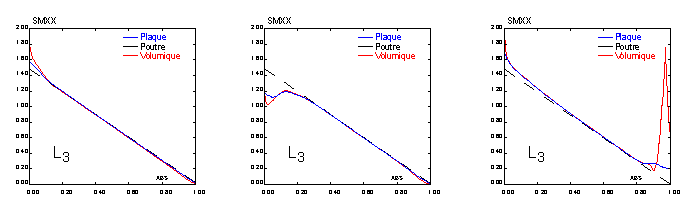
\includegraphics[height=45mm]{pout1-siglieux.eps}\\[-5mm]
\end{center}
\caption{\label{Pout1-siglieux} Contrainte axiale sur la peau supérieure en différentes sections}
\end{figure}
On y voit que loin des extrémités, les trois solutions concordent parfaitement, conformément 
au principe de Saint-Venant.\footnote{Le \textcolorblue{\textbf{principe de Saint-Venant}} précise que le comportement 
en un point quelconque de la poutre, pourvu que ce point soit suffisamment éloignédes zones 
d'applications des forces et des liaisons, est indépendant de la façon dont sont appliquées 
les forces et de la façon dont sont physiquement réalisées les liaisons; le comportement 
dépend alors uniquement du torseur des forces internes en ce point.}\index[aut]{Saint-Venant (Adhémar Jean Claude Barré de -), 1797-1886, Français}\index{Principe de Saint-Venant} 
Les différences proviennent des effets de bord, i.e. des variations 
locales des contraintes et déformations au voisinage des conditions aux limites.

Une comparaison plus fine des trois modélisations concernant cette même contrainte normale 
le long de trois lignes est reportée à la figure \ref{Pout1-sec}.

\medskip
Les différences de résultats proviennent des \textcolorred{hypothèses cinématiques} 
et des \textcolorred{composantes accessibles} dans les différentes théories utilisées.

\medskip
Les \textcolorblue{hypothèses cinématiques} sont:
\begin{figure}[ht]
\begin{center}
\includegraphics[height=25mm]{Pout1-Sec.eps}
\end{center}
\caption{\label{Pout1-sec} Mouvements d'une section droite: (a) théorie des poutres, 
(b) théorie des plaques ou coques, (c) théorie volumique.}
\end{figure}
\begin{itemize}
   \item la \textbf{théorie des poutres} (Figure \ref{Pout1-sec}a) suppose que chaque section droite 
	suit un mouvement de solide rigide. Les sections ne peuvent donc pas se déformer, 
	elles peuvent uniquement se translater et tourner dans l'espace (sans forcément rester 
	perpendiculaires à la ligne moyenne, car dans ce cas on considère une théorie avec 
	cisaillement transverse);
   \item la \textbf{théorie des plaques} (Figure \ref{Pout1-sec}b), moins restrictive, suppose que chaque 
	segment perpendiculaire au plan moyen de la plaque suit un mouvement de solide rigide 
	(là encore, sans forcément rester perpendiculaire au plan moyen). Elle permet donc de 
	modéliser certaines formes de déformations des sections, planes (flexion et cisaillement 
	dans le plan de la section, traction dans le sens de la largeur) ou hors plan (certains types 
	de gauchissement). Cependant, les segments ne pouvant pas changer de longueur, elle ne 
	permet pas de modéliser l'écrasement de l'épaisseur;
   \item enfin, la \textbf{théorie 3D} (Figure \ref{Pout1-sec}c) ne comporte aucune de ces restrictions et peut 
	modéliser n'importe quelle forme de gauchissement ou d'écrasement, à condition que le 
	maillage employé soit suffisamment fin.
\end{itemize}

\medskip
Ici, la comparaison des résultats <<~plaque~>> et <<~3D~>> montre que la contribution de 
l'écrasement de la section à la flèche semble négligeable (0,7\% d'écart).
Ce n'est pas forcément vrai car l'écrasement est un phénomène localisé sous la charge 
et lié au contact, qui a été modélisé très grossièrement... 
Cette très forte concentration de contraintes sous la charge est caractéristique d'une 
\textcolorred{singularité}. La valeur obtenue est peu fiable.
\textcolorgreen{On peut même dire que physiquement, une force ponctuelle n'existe pas. Elle est forcément
distribuée sur une petite surface...}


De même, la comparaison des résultats <<~poutre~>> et <<~plaque~>> montre que la flexion et le 
cisaillement de la section contribuent davantage à la flèche que l'écrasement (6,4\% d'écart): 
la largeur de la pièce est visiblement suffisante pour que les déformations des sections droites 
provoquent un déplacement vertical non négligeable sous la charge.

\medskip
Il est essentiel de noter que toutes les théories ne permettent pas d'accéder à toutes les 
composantes du champ des contraintes: de manière générale, seuls les efforts qui travaillent 
dans les déplacements permis par la théorie sont accessibles (les théories sont ainsi faites 
afin de pouvoir respecter le premier principe de la thermodynamique dont l'écriture nécessite 
de calculer le travail de tous les efforts permis par la théorie).
Les \textcolorblue{composantes accessibles} sont:
\begin{itemize}
   \item la \textbf{théorie des poutres} ne permet pas de calculer les contraintes dans le plan 
	transversal ($\sigma_{yy}$, $\sigma_{zz}$ et $\sigma_{yz}$) du fait de l'indéformabilité 
	des sections droites.;
   \item la \textbf{théorie des plaques} ne permet pas de calculer la contrainte normale au plan de la plaque 
	$\sigma_{zz}$, du fait de l'indéformabilité des segments perpendiculaires à ce plan ;
   \item enfin, la \textbf{théorie 3D} permet de calculer les six composantes du tenseur des contraintes.
\end{itemize}

\medskip
À ces limitations théoriques peuvent s'ajouter des \textcolorred{limitations techniques} 
propres à chaque logiciel, susceptibles de rendre d'autres grandeurs physiques inaccessibles. 
\textcolorgreen{Avant d'effectuer une modélisation par éléments finis, il est donc indispensable de 
s'assurer que le logiciel utilisé et son cadre théorique permettent bien d'accéder au résultat 
voulu} (en plus d'être pertinents vis-à-vis de la géométrie du produit, de son environnement 
et du comportement attendu).

De plus, si certains logiciels peuvent avoir des <<~limitations techniques~>>, ils peuvent
également disposer de \textcolorred{méthodes de post-traitement} susceptibles d'améliorer 
ou de permettre d'accéder à certaines composantes (sous certaines hypothèses). Cela aussi
doit être pris en compte.




\ifVersionAvecExemplesSepares\else
   \ifVersionAvecExemplesSepares
  \chapter{[\castem] Un calcul de poutre vu au chapitre~\ref{Ch-Model}}

  Nous allons reprendre pour partie l'exemple de la poutre encastrée traitée au chapitre~\ref{Ch-Model} sous \castem..
\else
  \section{Exemple: retour sur le calcul de poutre du paragraphe~\ref{Sec-champs} avec \castem}

  Nous allons reprendre pour partie l'exemple de la poutre encastrée traitée au paragraphe précédent et présenter
  le listing \castem correspondant.
\fi



\medskip
\ifVersionAvecExemplesSepares
  \section{Modélisation 2D}
\else
  \subsection{Modélisation 2D}
\fi

Nous commençons par définir les données du problème: longueur, largeur, épaisseur, nombre d'éléments
selon chacune de ces directions, et force appliquée:

\colorgris
\begin{Verbatim}[numbers=left,numbersep=3pt]
* DONNEES
* geometrie
long1=22.0;
larg1=8.;
ep1=4;
* maillage
nlong1=22;
nlarg1=8;
* effort
Forc1=-41.;
\end{Verbatim}
\colorblack

\medskip
Puis nous définissons la dimension du problème (modèle tridimensionnel), et le type de découpage:

\colorgris
\begin{Verbatim}[numbers=left,numbersep=3pt,firstnumber=last]
OPTION DIME 3 ELEM QUA4;
\end{Verbatim}
\colorblack

\medskip
Nous définissons les points~$k_i$ (dénommés ainsi pour rappel de la syntaxe Ansys des keypoints \verb|k,i,...|), puis les
lignes~$L_i$, et la surface~$S_1$.

\colorgris
\begin{Verbatim}[numbers=left,numbersep=3pt,firstnumber=last]
k1 = 0. 0. 0.;
k2 = long1 0. 0.;
k3 = long1 larg1 0.;
k4 = 0. larg1 0.;
*
L1 = DROI nlong1 k1 k2;
L2 = DROI nlarg1 k2 k3;
L3 = DROI nlong1 k3 k4;
L4 = DROI nlarg1 k4 k1;
*
S1 = DALLER L1 L2 L3 L4;
\end{Verbatim}
\colorblack

\medskip
Le modèle est un modèle de mécanique élastique isotrope utilisant lélément de coque COQ4 pour le maillage~$S_1$:

\colorgris
\begin{Verbatim}[numbers=left,numbersep=3pt,firstnumber=last]
Model1 = MODL S1 MECANIQUE ELASTIQUE ISOTROPE COQ4;
\end{Verbatim}
\colorblack

\medskip
Enfin on résout le problème après avoir fourni les données matérielles et les conditions aux limites:

\colorgris
\begin{Verbatim}[numbers=left,numbersep=3pt,firstnumber=last]
Mater1 = MATERIAU Model1 YOUNG 70000.0 NU 0.33 RHO 2700.0;
Car1 = CARAC Model1 EPAI ep1;
Mater1 = Mater1 ET Car1;
MR1 = RIGIDITE Model1 Mater1;
CL1 = BLOQ DEPL L4;
CL2 = BLOQ ROTA L4;
FOR1 = FORCE(0. 0. Forc1) k3;
MTOT1 = MR1 ET CL1 ET CL2;
Depl1 = RESOUD MTOT1 FOR1 ;
\end{Verbatim}
\colorblack

\medskip
On peut post-traiter les résultats et les afficher.

Les composantes de~$Sig_1$ dans le repère LOCAL sont:
\begin{itemize}
  \item les efforts normaux: N11, N22;
  \item l'effort de cisaillement plan: N12; 
  \item les moments de flexion: M11, M22;
  \item le moment de cisaillement plan: M12;
  \item les efforts tranchants V1, V2.
\end{itemize}

Les composantes de~$Eps_1$ dans le repère LOCAL sont:
\begin{itemize}
  \item les élongations normales dans le plan: EPSS, EPTT;
  \item les cissions dans le plan et transverses: GAST, GASN, GATN;
  \item les courbures: RTSS, RTTT, RTST.
\end{itemize}

\colorgris
\begin{Verbatim}[numbers=left,numbersep=3pt,firstnumber=last]
* DEPLACEMENTS
UZ1 = EXCO 'UZ' depl1;
*TRAC UZ1 S1;
*
* DEFORMEE
def0 = DEFO S1 Depl1 0.0 BLEU;
def1 = DEFO S1 Depl1;
*TRAC (def0 ET def1);
*
* CONTRAINTES: 
Sig1 = SIGM Model1 Mater1 Depl1;
Siigg1 = EXCO M11 Sig1;
TRAC Siigg1 Model1 def1;

* DEFORMATIONS
Eps1 = EPSI Model1 Mater1 Depl1;
Eppss1 = EXCO RTSS Eps1;
*TRAC Eppss1 Model1;

fin;
\end{Verbatim}
\colorblack


\medskip
\ifVersionAvecExemplesSepares
  \section{Modèle 3D}
\else
  \subsection{Modèle 3D}
\fi

Nous allons maintenant construire le modèle tridimensionnel.

Comme nous voulons travailler à l'économie, nous repartons du fichier précédent que nous adaptons.

\colorgris
\begin{Verbatim}[numbers=left,numbersep=3pt]
* DONNEES
* geometrie
long1=22.0;
larg1=8.;
ep1=2;
* maillage
nlong1=22;
nlarg1=8;
nep1=3;
* effort
Forc1=-41.;
\end{Verbatim}
\colorblack

\medskip
Cette fois, nous nous servons de CUB8 au lieu de QUA4.

\colorgris
\begin{Verbatim}[numbers=left,numbersep=3pt,firstnumber=last]
OPTION DIME 3 ELEM CUB8;
*
k1 = 0. 0. 0.;
k2 = long1 0. 0.;
k3 = long1 larg1 0.;
k4 = 0. larg1 0.;
*
L1 = DROI nlong1 k1 k2;
L2 = DROI nlarg1 k2 k3;
L3 = DROI nlong1 k3 k4;
L4 = DROI nlarg1 k4 k1;
*
S1 = DALLER L1 L2 L3 L4;
\end{Verbatim}
\colorblack

\medskip
À partir de la surface~$S_1$, qui est la même que précédemment, nous allons créer le volume~$V_1$ par translation
selon le vecteur~$Vect_1$.

Nous en profitons également pour créer~$Face_1$ sur laquelle porterons les conditions aux limites.
Notons par exemple que la ligne~$L_4$ appartient bien au maillage~$V_1$, puisque ce dernier est construit dessus.
Par contre, la surface~$face_1$ n'appartient pas à~$V_1$, il est donc nécessaire de la lier à~$V_1$ en utilisant
la commande ELIM.

\colorgris
\begin{Verbatim}[numbers=left,numbersep=3pt,firstnumber=last]
Vec1=0. 0. (-1.0*ep1);
V1=S1 VOLU nep1 TRAN Vec1;
Face1 = L4 TRAN nep1 Vec1;
ELIM 0.0000001 V1 Face1;
\end{Verbatim}
\colorblack

\medskip
Cette fois, le modèle correspond au maillage~$V_1$ et utilise l'élément CUB8.

\colorgris
\begin{Verbatim}[numbers=left,numbersep=3pt,firstnumber=last]
Model1 = MODL V1 MECANIQUE ELASTIQUE ISOTROPE CUB8;
\end{Verbatim}
\colorblack

\medskip
On résout, puis on post-traite.

\colorgris
\begin{Verbatim}[numbers=left,numbersep=3pt,firstnumber=last]
Mater1 = MATERIAU Model1 YOUNG 70000.0 NU 0.33 RHO 2700.0;
MR1 = RIGIDITE Model1 Mater1;
CL1 = BLOQ DEPL Face1;
CL2 = BLOQ ROTA Face1;
FOR1 = FORCE(0. 0. Forc1) k3;
MR1 = MR1 ET CL1 ET CL2;
Depl1 = RESOUD MR1 FOR1 ;
*
* DEPLACEMENTS
UZ1 = EXCO 'UZ' depl1;
*TRAC CACH UZ1 V1;
* DEFORMEE
def0 = DEFO V1 Depl1 0.0 BLEU;
def1 = DEFO V1 Depl1;
*TRAC CACH (def0 ET def1);
*
* CONTRAINTES: 
Sig1 = SIGM Model1 Mater1 Depl1;
* Les composantes de Sig1 sont: VONMISES, SMXX, SMYY, SMZZ, SMXY, SMXZ, SMYZ
Siigg1 = EXCO SMXX Sig1;
* on trace sur la geometrie deformee, c'est plus beau
TRAC CACH Siigg1 Model1 def1;
*
* DEFORMATIONS
*Eps1 = EPSI Model1 Mater1 Depl1;
*TRAC CACH Eps1 Model1;

fin;
\end{Verbatim}
\colorblack
% poutre Ch 10 sous Cast3M
%   \section{Exemple: calcul des effort équivalents pour une poutre}

  Dans ce paragraphe, et pour poursuivre notre illustration des différentes modélisation d'un même problème, nous présentons 
  un petit calcul de RdM traité selon l'approche mécanicienne.

  Il permet de montrer comment sont calculés les efforts équivalents, dans un cas général, sur une poutre, mais le
  même type de calcul resterait valable pour tout type d'élément.

\medskip
\subsection{Problème}

\medskip
Considérons une poutre définie dans son système de coordonnées locales comme montré à la figure 
ci-dessous:
%Let us consider a member defined in its local coordinates system, as shown
%above in \fig{beam1}.
%
%
%\begin{figure}[ht]
 \begin{center}
 \begin{picture}(250,60)(-10,-35)
 %F,F1,F2
  \thicklines
  \put(100,25){P(x)}
  \put(0,25){\vector(0,-1){25}}
  \put(200,25){\vector(0,-1){25}}
  \put(-15,25){F}
  \put(-8,20){1}
  \put(205,25){F}
  \put(212,20){2}

 %C1,C2
  \put(0,0){\oval(20,20)[lt]}
  \put(0,0){\oval(20,20)[rt]}
  \put(0,0){\oval(20,20)[rb]}
  \put(0,-10){\vector(-1,0){6}}
  \put(10,-15){C}
  \put(17,-20){1}
  \put(200,0){\oval(20,20)[lt]}
  \put(200,0){\oval(20,20)[rt]}
  \put(200,0){\oval(20,20)[rb]}
  \put(200,-10){\vector(-1,0){6}}
  \put(180,-15){C}
  \put(187,-20){2}

 %axes
  \thinlines
  \put(0,-15){\line(0,1){30}}
  \put(0,0){\vector(0,-1){35}}
  \put(-10,-35){y}
  \put(0,0){\vector(1,0){235}}
  \put(230,-10){x}

 %Load
  \bezier{180}(0,10)(30,25)(60,15)
  \bezier{240}(60,15)(100,5)(140,20)
  \bezier{180}(140,20)(170,23)(200,18)

 %encastrement
  \multiput(-4,-20)(0,8){5}{/}
  \multiput(200,-20)(0,8){5}{/}
  \put(200,-22){\line(0,1){40}}

 %beam
  \linethickness{3pt}
  \put(0,0){\line(1,0){200}}
 \end{picture}
 \end{center}
% \label{beam1}
% \caption{Considered beam and its local coordinates system}
%\end{figure}

La première extrémité est~$\left( 0,0,0\right)~$ et la seconde~$\left( l,0,0\right)~$, 
où~$l$ est la longueur de la poutre.

Nous supposerons la poutre encastrées aux deux bouts, et soumise à une charge
distribuée définie par la fonction~$P(x)$.

Le problème est plan de sorte que~$\overrightarrow{P(x)}
=P(x)\overrightarrow{y}$

Nous souhaitons déterminer les forces et moments équivalents~$F_1$, $F_2$ et
$C_1$, $C_2$ aux deux extrémités également appelées nœuds 1 et 2.

\medskip
Une analyse statique conduit à:

\begin{quotation}
\begin{equation}
  \label{staticF}
  F_1+F_2+\int_0^l P(x)dx=0 
\end{equation}

\begin{equation}
  \label{staticC}
  C_1+C_2+F_2l+\dint_0^l x P(x)dx=0 
\end{equation}
\end{quotation}


\medskip
Le moment de flexion s'exprime:

\begin{quotation}
$M_z(x)=C_1-F_1x-\dint_0^x x P(x)dx$, ou

$M_z(x)=-C_2-F_2(l-x)-\dint_x^l(v-x) P(x)dv$
\end{quotation}

\medskip
L'énergie interne de la poutre s'esprime:
%The beam's internal energy can be explained as follows~:

%\begin{quote}
\[
\delta J=\frac 12\dint_0^l\dfrac{M_z^2(x)}{EI}dx
\]
%\end{quote}

\medskip
\subsection{Théorème de Menabrea}\index[aut]{Menabrea (Luigi Federico; général comte -; premier marquis de Valdora), 1867-1869, Italien}\index{théorème!de Menabrea}

Le théorème de Menabrea permet d'écrire:

\begin{quotation}
 ~$\dfrac{\partial \delta J}{\partial C_1} =
  \dfrac{\partial \delta J}{\partial C_2} =
  \dfrac{\partial \delta J}{\partial F_1} =
  \dfrac{\partial \delta J}{\partial F_2} = 0$
\end{quotation}

Ces calculs seront faits après avoir introduit les notations suivantes:
\begin{quotation}\colorblue
 ~$I_0(a,b)=\dint_a^b P(x)dx$

 ~$I_1(a,b)=\dint_a^b x P(x)dx$
\end{quotation}\colorblack


$\dfrac{\partial \delta J}{\partial C_1}=0$~:

\begin{quotation}
$\qquad \dint_0^lM_z(x)dx=0$

$\qquad \dint_0^lC_1-F_1x-I_1(0,x)dx=0$
\end{quotation}

\begin{equation}
  \label{MenaC}
  C_1l-\frac 12F_1l^2-\int_0^lI_1(0,x)dx=0
\end{equation}

$\dfrac{\partial \delta J}{\partial F_1}=0$~:

\begin{quotation}
$\qquad \dint_0^lxM_z(x)dx=0$

$\qquad \dint_0^lC_1-F_1x-I_1(0,x)dx=0$
\end{quotation}

\begin{equation}
  \label{MenaF}
  C_1l-\frac 12F_1l^2-\int_0^lI_1(0,x)dx=0
\end{equation}

Nous utilisons les propriétés des intégrales précédemment définies:

\begin{quotation}
$I(a,b)=I(a,c)+I(c,b)$

$I(b,a)=-I(a,b)$
\end{quotation}

for both~$I_0$ and~$I_1$.


\medskip
\subsection{Résolution des équations}

En utilisant ($\ref{MenaC}$) et ($\ref{MenaF}$), on trouve~$F_1$ and~$C_1$,
Puis, en utilisant ($\ref{staticF}$) et ($\ref{staticC}$) on obtient~$F_2$ and~$C_2$.

Les efforts sont:

\begin{quotation}
$F_1=\dfrac 6{l^2}\left( \dint_0^lI_1(0,x)dx-\frac
2l\dint_0^lxI_1(0,x)dx\right)~$

$F_2=-I_0(0,l)-F_1$

$C_1=\dfrac 2l\left( 2\dint_0^lI_1(0,x)dx-\dfrac
3l\dint_0^lxI_1(0,x)dx\right)~$

$C_2=\dfrac 2l\left( \dint_0^lI_1(0,x)dx-\dfrac
3l\dint_0^lxI_1(0,x)dx\right) +lI_0(0,l)-I_1(0,l)$
\end{quotation}

\medskip
\subsection{Conclusion}

Ces forces et moments correspondent à des éléments finisforts de réactions.
Les forces équivalentes utilisées en MEF correspondent aux efforts internes
développés dans la poutre. Ce sont:

\begin{tabbing}
  at node iiiiii\=Forceqqq\= \kill
       \>Force \>Moment\\
  Au nœud 1 \> ~$-F1$ \> ~$-C1$\\
  Au nœud 2 \> ~$-F2$ \> ~$-C2$\\
\end{tabbing}

Analytiquement:

\begin{equation}\colorblue
\label{Feq}\left\{
\begin{array}{l}
  F_1=-\dfrac 6{l^2}\PP{\dint_0^lI_1(0,x)dx-\dfrac 2l\dint_0^lxI_1(0,x)dx} \\
  F_2=I_0(0,l)-F_1 \\
  C_1=-\dfrac 2l\PP{2\dint_0^lI_1(0,x)dx-\dfrac3l\dint_0^lxI_1(0,x)dx} \\
  C_2=-\dfrac 2l\PP{\dint_0^lI_1(0,x)dx-\dfrac3l\dint_0^lxI_1(0,x)dx}
  -lI_0(0,l)+I_1(0,l)
\end{array}
\right.
\end{equation}\colorblack
et sous forme vectorielle:

\begin{quotation}
$\left\{
\begin{array}{l}
  \overrightarrow{F_1}=F_1\overrightarrow{y} \\
  \overrightarrow{F_2}=F_2\overrightarrow{y} \\
  \overrightarrow{C_1}=C_1\overrightarrow{z} \\
  \overrightarrow{C_2}=C_2\overrightarrow{z}
\end{array}
\right.~$
\end{quotation}


% efforts équivalents sur une poutre
\fi

\medskip
\section{Interpolation des champs et de la géométrie}

Un élément est dit \textcolorblue{isoparamétrique} si on prend les mêmes fonctions 
d'interpolation pour le déplacement et la géométrie.

De manière évidente, on définit également les éléments super et sous-paramétriques,
comme illlustré à la figure \ref{EFnonISO}.
\begin{figure}[ht]
\begin{center}
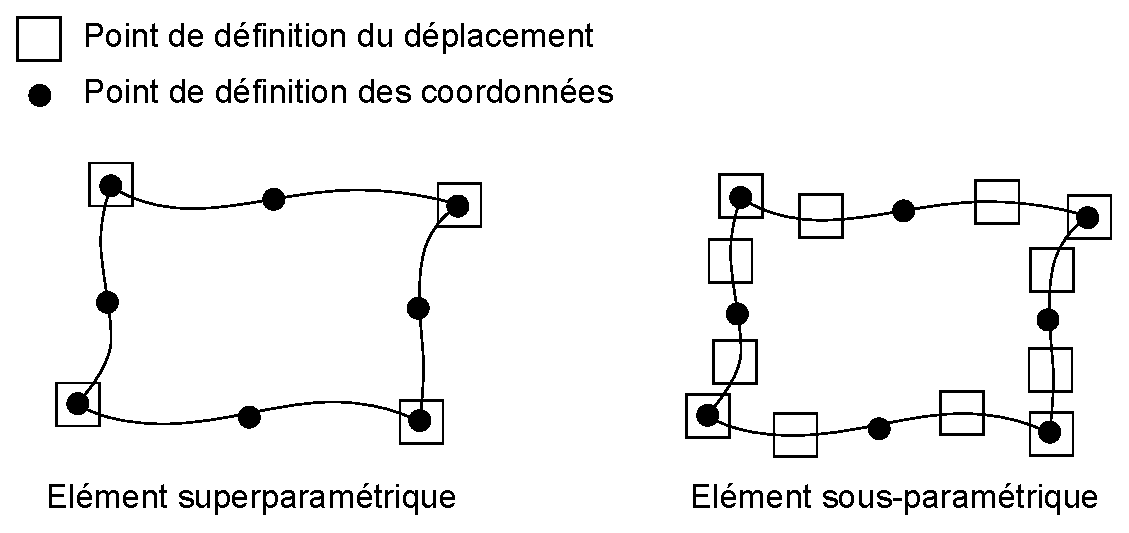
\includegraphics[height=45mm]{EFnonISO.eps}
\end{center}
\caption{\label{EFnonISO} éléments finis non isoparamétriques.}
\end{figure}

\textcolorgreen{Ceci est juste une remarque en passant, pour définir le
vocabulaire en somme, nous n'en reparlerons plus dans la suite du document.}
